\section{Numerical stability and reproducibility}
\label{sec:C07:numerics}
Mixed precision changes the numerical contract. Lower-precision matrix multiplication can provide high throughput, while accumulation, normalization, optimizer updates, and reductions may require higher precision. Dynamic loss scaling can prevent small gradients from underflowing but does not solve every overflow or instability. Gradient clipping changes the update and should be reported with its norm convention and distributed aggregation. A local shard norm is not generally the global gradient norm. For a disjoint partition $\mathcal S$ of logical gradient coordinates, $\|g\|_2^2=\sum_{S\in\mathcal S}\sum_{i\in S}g_i^2$; replicated copies must not be counted as additional coordinates. The inspected Stage-3 \path{get_grad_norm_direct} uses parameter-ownership predicates and configured partition/model/expert reductions, rather than simply summing every resident tensor~\cite{repo_deepspeed}. Testing the norm therefore requires the actual replication and process-group map as well as the tensor values. Incorrect clipping across parallel groups can create a different optimizer even when the learning-rate schedule is unchanged.

Randomness includes initialization, dropout, data order, sampling, and distributed execution choices. Saving a seed without generator state and data-loader position is insufficient for exact resumption. Some kernels are nondeterministic, and changing the number of ranks can change reduction order and sample assignment. Reproducibility should distinguish bitwise replay from statistical agreement of learning curves and downstream outcomes. The latter still requires enough repeated runs or a justified uncertainty analysis. A single expensive pretraining run provides limited evidence about sensitivity to optimization randomness.

Checkpoint integrity requires a consistent snapshot of weights, optimizer state, scheduler, random generators, data progress, and partition metadata. A partial write can leave shards individually readable but mutually inconsistent. Use a manifest that binds expected shards and checksums, with a commit marker written only after all required state is durable. Recovery should verify the manifest before constructing a model. This is a systems property that can be tested through fault injection: interrupt saves, remove a shard, alter a checksum, or resume under an incompatible parallel layout and confirm explicit failure or documented conversion.

Training-service monitoring should distinguish transient hardware errors from statistical divergence. Loss spikes, gradient norm changes, nonfinite values, data anomalies, and communication retries carry different evidence. Automatically discarding a spike can hide a genuine data-quality problem; automatically restarting from the same checkpoint can repeat the same deterministic failure. A recovery policy should retain the offending batch identity and numerical context where permitted. Otherwise the system can consume substantial compute without resolving the underlying issue, while the final report shows only the successful resumed segment.

\paragraph{Unequal sequence lengths can silently change the objective.}
Suppose rank $j$ has $B_j$ supervised tokens after masking and computes a local mean loss $L_j$. Averaging those local means across $n$ ranks gives $n^{-1}\sum_jL_j$. The intended global token mean is instead $\sum_j B_jL_j/\sum_jB_j$. They agree only under special conditions, such as equal supervised-token counts or identical local losses. The same discrepancy applies to gradients. Variable-length agent traces, tool-observation masks, and uneven packing make this more than a theoretical corner case: short traces can receive disproportionate weight when each rank normalizes locally before an unweighted average.

The correction is to aggregate the appropriate numerator and denominator or scale local contributions consistently with the collective's averaging convention. Gradient accumulation adds another level. If microbatch $k$ on rank $j$ contains $B_{jk}$ supervised tokens, dividing every microbatch loss by a fixed accumulation count does not implement the global token mean when these counts differ. The correct relative contribution is proportional to $B_{jk}$ for a token-weighted objective. A sequence-weighted objective is also legitimate, but must be intentional and implemented consistently. The distinction changes how long reasoning traces and short tool calls influence the learned policy.

A minimal verification uses a tiny deterministic model and two microbatches with deliberately unequal mask counts. Compute one reference gradient on their concatenation under the intended objective. Compare it with gradients from the distributed or accumulated path before the optimizer step. Repeat with a fully masked microbatch, which should have defined behavior rather than division by zero, and with uneven examples across ranks. This test is meaningful because it checks a mathematical objective independently of a large model's apparent convergence. A training curve can look normal while optimizing the wrong weighting of trace types.

Another useful check separates clipping from averaging. Clipping each microbatch gradient before accumulation generally differs from clipping the final accumulated gradient because clipping is nonlinear. Likewise, clipping each rank's local gradient differs from clipping the global combined gradient. Either policy can be chosen, but it changes the optimizer and its stability behavior. Record where loss scaling, unscaling, accumulation, reduction, and clipping occur. These details are particularly important when a post-training stage mixes long-horizon action trajectories with short preference examples on the same distributed infrastructure.

The numerical and causal contracts meet at the masked token. Its target, visibility, weight, and distributed contribution all determine the update. A trace that is causally correct but incorrectly normalized can bias learning toward an unintended task mixture. A numerically correct all-reduce cannot repair future-information leakage in the local batch. Auditing both layers produces a stronger interpretation of downstream agent gains than treating data preparation and infrastructure as independent implementation details.

For an averaging collective, the accumulation can be specified directly as a token-weighted gradient. Let $\theta\in\mathbb R^p$, with $p\geq1$. On rank $j\in\{1,\ldots,n\}$, let $k\in\{1,\ldots,K_j\}$ index microbatches and $i\in I_{jk}$ their token positions. Let $a_{jki}\in\{0,1\}$ be a fixed authoritative supervision mask and $\ell_{jki}(\theta)$ the corresponding differentiable token loss. The window defines
\begin{equation}
\label{eq:C07:masked-window}
\begin{aligned}
 B&=\sum_{j=1}^{n}\sum_{k=1}^{K_j}\sum_{i\in I_{jk}}a_{jki},\\
 N_{jk}(\theta)&=\sum_{i\in I_{jk}}a_{jki}\ell_{jki}(\theta),\\
 L(\theta)&=\frac1B\sum_{j=1}^{n}\sum_{k=1}^{K_j}N_{jk}(\theta),
 \qquad B>0.
\end{aligned}
\end{equation}
All contributions are differentiated at the same parameter snapshot $\theta_t$. With no additional microbatch normalization, the local and collective updates are
\begin{equation}
\label{eq:C07:global-gradient}
\begin{aligned}
 g_{j,0}&=\mathbf0,\\
 g_{j,k}&=g_{j,k-1}+\frac nB\nabla_\theta N_{jk}(\theta_t),\\
 g_t&=\frac1n\sum_{j=1}^{n}g_{j,K_j}
     =\nabla_\theta L(\theta_t).
\end{aligned}
\end{equation}
For a collective that sums rather than averages, replace $n/B$ by $1/B$ and remove the outer $1/n$. A fully masked window has $B=0$ and is rejected before this update is defined; it does not invoke the optimizer transition below. A fully masked microbatch within a valid window contributes the zero numerator without introducing a local division by zero.

Let $z_t=(\theta_t,\omega_t)\in\mathbb R^p\times\Omega$ include the declared optimizer state $\omega_t\in\Omega$. For finite $g\in\mathbb R^p$, a global norm limit $c\in(0,\infty]$ gives the optional clipping map and optimizer transition
\begin{equation}
\label{eq:C07:clipped-update}
\begin{aligned}
 \mathcal K_c(g)&=\begin{cases}
 g,&\|g\|_2\leq c,\\
 c\,g/\|g\|_2,&\|g\|_2>c,
 \end{cases}\\
 z_{t+1}&=\mathcal U_t\!\left(z_t,\mathcal K_c(g_t)\right).
\end{aligned}
\end{equation}
The choice $c=\infty$ disables clipping, and $\mathcal K_c(\mathbf0)=\mathbf0$ without a division by zero. The operator $\mathcal U_t$ is the configured optimizer, not an assumption of plain gradient descent. A zero input gradient can still change weights or optimizer state through momentum, weight decay, or step counters; it differs from rejecting a window without invoking $\mathcal U_t$. The gradient identity holds in exact arithmetic with fixed masks; loss scaling must be undone consistently, and rounding, reduction order, and backend accumulation behavior require the preceding implementation checks.



Figure~\ref{fig:C07:token-weighting} isolates the mechanism and its stated information boundaries.
\begin{figure}[!htbp]
\centering
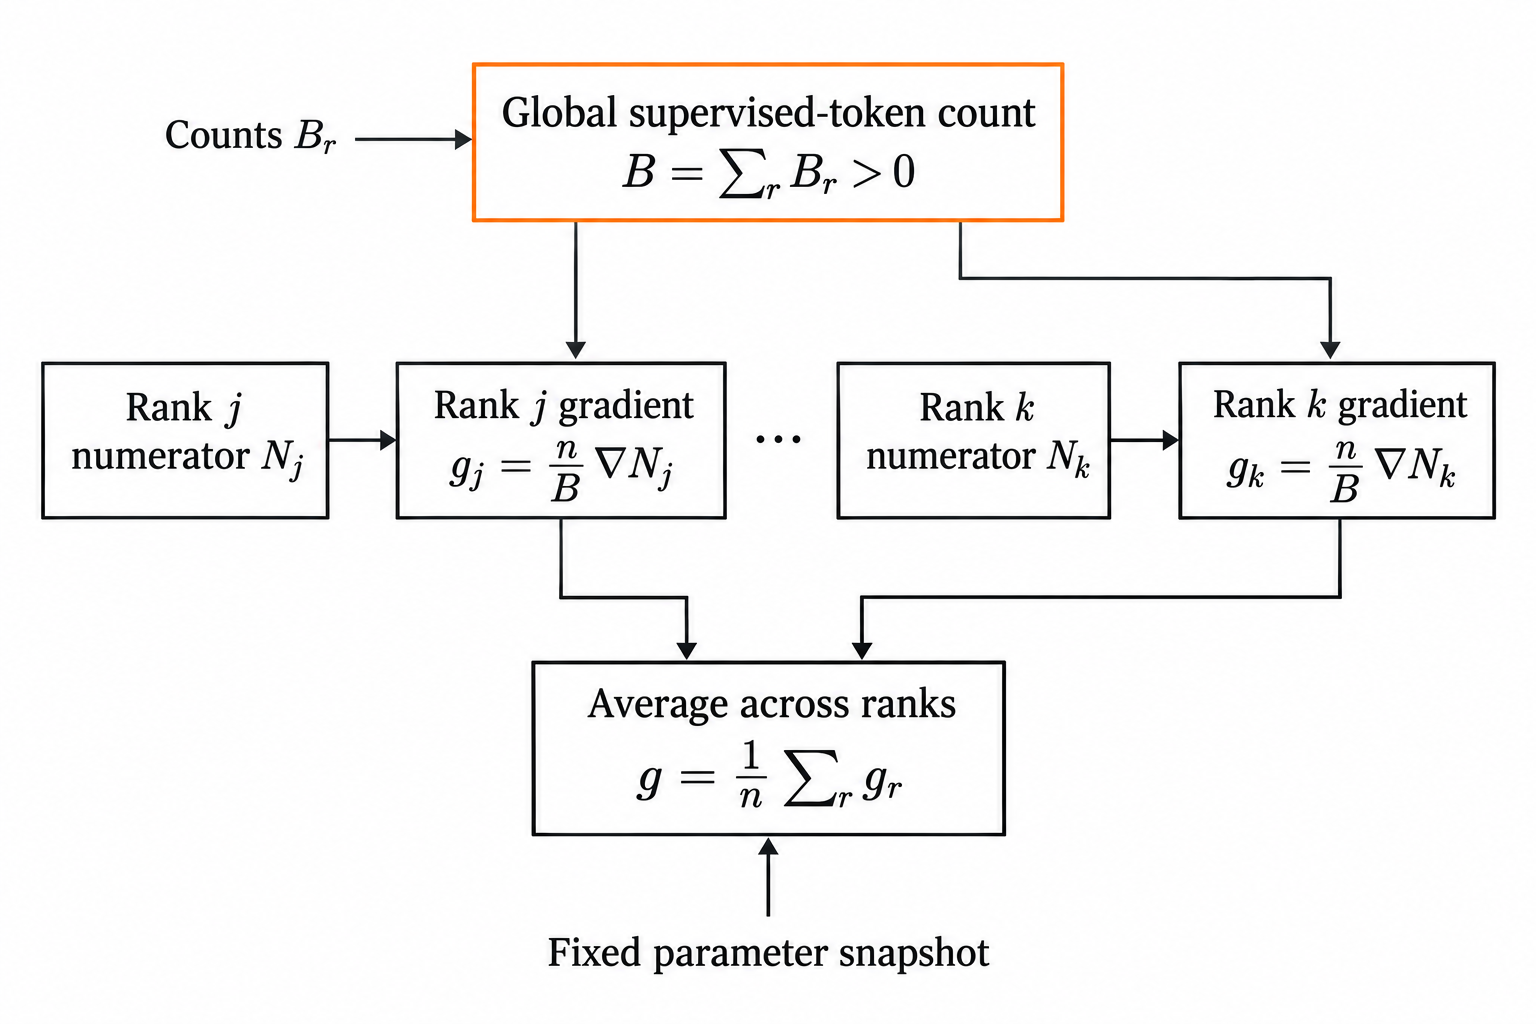
\includegraphics[width=\linewidth]{book/figures/assets/F07review.png}
\caption{Token-weighted accumulation requires one global normalization. At a common parameter snapshot, rank $j$ contributes token-loss numerator $N_j$ and supervised-token count $B_j$. For $B=\sum_jB_j>0$, scaling by $n/B$ and an averaging collective yields $\nabla[(\sum_jN_j)/B]$. Counts are fixed batch metadata; the snapshot condition applies to every rank gradient. Locally normalized means generally define a different objective. No training measurement is depicted.}
\label{fig:C07:token-weighting}
\end{figure}
